\chapter{Methods}
\section{Water Year 2019} 
\subsection{Thermocouple Array}
Our temperature sensor is located at Banner Creek Summit in central Idaho. This location has an elevation of about 7,040 feet above sea level and is proximal to Idaho State Highway 21. The area around Banner Summit receives an average of 1.9 meters of snow each year and frequently experiences extreme low temperatures as low as -40\textdegree C. The 2018 -- 2019 winter season experienced an above-average snowfall, with a peak snow water equivalent (SWE) measured at Banner Summit at 120\% of average. Site visits occured on a biweekly basis unless weather or road closures forbid access. During each visit, data was collected from the instrument and snow samples were collected for stable water isotope analysis.

The structure of our sensor is comprised of a steel, rectangular frame with thin, metal cables running horizontally in 5cm increments (Fig. \ref{fig:Banner_Sensor}). A single Omega Type T thermocouple is attached to each wire, a quarter distance between the two support posts, which forms a vertical array of temperature sensors spaced 5cm apart, up to 2.5m above the ground. There were two thermocouples buried in the soil at 10cm and 5cm below ground. The buried 10cm thermocouple was installed directly adjacent to a thermistor (Campbell Scientific T107). The 53 thermocouples were multiplexed using a Campbell Scientific AM32 to a Campbell Scientific CR1000 data logger. Temperature measurements were recorded every 5 minutes. The design for this sensor came from Charlie Luce and Tom Black at the USFS and it was based off an existing sensor installed at Bogus Basin, near Boise, ID. 

A Micro-Specialties satellite telemetry system was installed during the 2020 water year so that data were accessible in near-real time. Data was transmitted every six hours using an hourly average from the measurements taken the hour before each transmit.

 \begin{figure}[H]
    \centering
    \includegraphics[width=0.7\linewidth]{figures/Banner_Sensor.jpeg}
    \caption{Picture of the instrument installed at Banner Creek Summit.}
    \label{fig:Banner_Sensor}
 \end{figure}
 
\subsection{Temperature Gradient Analysis}
The temperature gradient analysis focuses on three subsets from the 2018--2019 winter season. These three subsets are selected because they illustrate critical elements of how temperature gradients evolve throughout the season. An early-season subset between November 31 to December 28 shows large temperature gradients throughout the shallow snowpack; observations made in snowpits on these two dates indicate depth hoar formation. A mid-season subset during February shows extreme cold events and record amounts of snowfall; the lowest portion of the snowpack is well insulated and does not experience critical temperature gradients. The late-season subset during March shows the snowpack as it reaches isothermal conditions.  

Temperature gradients at the top of the snowpack change diurnally because it is not completely insulated from the air. In cold, alpine environments such as Banner Summit, there was often extreme temperature gradients in the top 25cm that can lead to the formation of faceted snow. However, the diurnal nature of the upper 25cm often means that critical temperature gradients are not sustained long enough to produce faceted snow forms. The below analysis focuses on the upper 25cm because this is the extent of solar radiation penetration into the snowpack.  

In this analysis, we calculated the hourly average temperature gradients in the upper 25cm and the lowest 20cm of the snowpack using a first-order polynomial regression between depth and temperature (Figure \ref{fig:TempGrad_Ex}). This was done in MATLAB using the built in function called polyfit.  Data in the upper 25cm are selected because solar radiation penetrates between ~20 - 30cm depth. The snow surface for the upper 25cm calculation is measured by the nearby SNOTEL site. The slope of each polynomial, i.e., the temperature gradients during 2019 in the upper 25cm and lowest 20cm, are shown in Figures \ref{fig:WY2019_L20_Grad} - \ref{fig:Mar_L20_RDH}.  

\begin{figure}[H]
    \centering
    \includegraphics[width=0.5\linewidth]{figures/TempGrad/TempGrad_Ex.eps}
    \caption{Example of a first order regression fit to the upper 25cm and lowest 20cm. The snow surface, as measured by the Banner Summit SNOTEL site is the horizontal, dark gray line which marks the upper limit (snow depth) of the upper 25 cm interval.}
    \label{fig:TempGrad_Ex}
\end{figure}

\subsection{Stable Water Isotopes}
Snow was sampled within 20 meters of the Banner Summit SNOTEL site for analysis of stable water isotopes. The snow pit locations are randomly selected on a flat surface with no apparent aspect. The sampled area is lightly forested, but care is taken in order to prevent contamination from secondary snow input such as fallen, intercepted snow or wind drifts. In order to capture the full isotopic content of a snowpack, samples were collected from the whole snow profile with a 3cm vertical resolution. To assess spatial variability of stable water isotopes, duplicate samples were collected from one pit with about 0.5 m horizontal spacing (figure \ref{fig:Pit_18Dec19}). To assess systematic bias in the sampling method, samples were collected in triplicates directly adjacent to each other (figure \ref{fig:Pit_17Mar19}). Detailed notes are taken on snowpack characteristics during each sampling event.

Snow samples are transported back to Boise State University where they are stored at -20°C. A fourth generation (purchased 2011) Los Gatos Research (LGR) Liquid Water Isotope Analyzer (LWIA) is used to measure \textsuperscript{2}H/\textsuperscript{1}H and \textsuperscript{18}O/\textsuperscript{16}O for all snow samples. Results are reported in units of per mil (\textperthousand), relative to Vienna Standard Mean Ocean Water (VSMOW). Raw LWIA values are processed using the Los Gatos Research post-processing software.

 \begin{figure}[H]
    \centering
    \includegraphics[width=0.4\linewidth]{figures/Pit_18Dec19.png}
    \caption{Picture of the sampling pit used on December 18, 2018 illustrating where duplicates were sampled with about 0.5m spacing as represented by the shaded boxes with black lines. The red and green dots are observed ice layers, and storm layer surfaces.}
    \label{fig:Pit_18Dec19}
 \end{figure}
 
 \begin{figure}[H]
    \centering
    \includegraphics[width=0.3\linewidth]{figures/Pit_17Mar19.jpg}
    \caption{Picture of the sampling pit used on March 17th, 2019 showing where triplicates were collected.}
    \label{fig:Pit_17Mar19}
 \end{figure}
 
 